% !TEX encoding = UTF-8 Unicode
\documentclass[a4paper,12pt]{article}

%-----------------------------------------Include package & set up some thing-----------------------------------------------
\usepackage{fontspec}
\setmainfont{Times New Roman} %set font
\usepackage{enumitem} % to format list
\usepackage{amsmath}
\usepackage{listings} % quote code
\usepackage{color}
\usepackage{hyperref} % cite hyperlink & bookmarks
\usepackage{setspace} % space
\usepackage{graphicx} % insert image
\usepackage{subcaption} % Multiple images
\usepackage{float}
\usepackage[margin=1in, footskip = 0.25in]{geometry} % Change margin with geometry package

\hypersetup{unicode, colorlinks,linkcolor=black, urlcolor=cyan} % format hyperlink and bookmarks

%Define title
\title{Báo cáo bài tập 6}
\author{1612174 - Phùng Tiến Hào - \href{mailto:tienhaophung@gmail.com}{tienhaophung@gmail.com}}
\date{05/05/2019}

%Code formatting with the listing package
\definecolor{codegreen}{rgb}{0,0.6,0}
\definecolor{codegray}{rgb}{0.3,0.3,0.3}
\definecolor{codepurple}{rgb}{0.58,0,0.82}
\definecolor{backcolour}{rgb}{0.92,0.92,0.88}

\lstdefinestyle{mystyle}{
	backgroundcolor=\color{backcolour},   
	commentstyle=\color{codegreen},
	keywordstyle=\color{blue},
	numberstyle=\tiny\color{codegray},
	stringstyle=\color{codepurple},
	basicstyle=\footnotesize,
	breakatwhitespace=false,         
	breaklines=true,                 
	captionpos=b,                    
	keepspaces=true,                 
	numbers=left,                    
	numbersep=5pt,                  
	showspaces=false,                
	showstringspaces=false,
	showtabs=false,                  
	tabsize=2,
	columns=fullflexible,
	frame=single
}

\lstset{style=mystyle}

\begin{document}
	\pagenumbering{gobble}
	\maketitle
	\newpage
	
	\doublespacing
	\tableofcontents
	\singlespace
	
	\newpage
	\pagenumbering{arabic}
	
	\textbf{Dữ liệu khảo sát:} SpeedDating trong package Lock5withR\\
	
	Load package và thêm các thư viện cần thiết trước khi đi vào xử lý:
	\begin{lstlisting}[language=R]
	require(Lock5withR) # Load package
	library(Lock5withR)
	library(mosaic)
	head(SpeedDating)
	attach(SpeedDating) # Avoid dollar sign before each varibles name
	\end{lstlisting}
	\section{Khảo sát một biến}
	\subsection{Biến định tính (Categorical variable)}
	\subsubsection{DecisionMale (Yes/No)}
	Giả sử, ta cần khảo sát tỉ lệ nam phản hồi (Yes/No) cho quần thể (population) là toàn bộ học sinh nam của trường Columbia. Từ tổng thể, ta thu thập được một mẫu dữ liệu ngẫu nhiên (random sample) gồm 276 quan sát trong đó có 146 phản hồi "Yes" và 130 phản hồi "No". Dựa vào mẫu dữ liệu này, ta kiểm định nghi vấn "tỉ lệ phản hồi Yes cao hơn phản hồi No" với mức ý nghĩa (significance level) 5\%.
	
	Gọi $p$ là tỉ lệ nam phản hồi "Yes" trong trường, $\hat{p}$ là tỉ lệ nam phản hồi "Yes" trong mẫu dữ liệu. Ta có
	$$\hat{p} = \frac{146}{276} = 0.529$$
	
	Để tính đến sự biến động của $\hat{p}$ theo mẫu dữ liệu $n = 276$ thu thập từ tổng thể, ta thực hiện kiểm định giả thuyết:
	
	\begin{equation*}
		\begin{cases}
		H_0: p = p_0 = 0.5\\
		H_1: p > 0.5
		\end{cases}
	\end{equation*}
	với mức ý nghĩa $\alpha = 0.5\%$
		
	\begin{lstlisting}[language=R]
	# TK can tinh
	stat <- function(data){
		return (mean(data == "Yes")) # Ti le
	}
	
	randomization <- function(B){
		return (replicate(B, stat(sample(nullsample, n, replace = TRUE))))
	}
	
	> # Mau du lieu ban dau
	> sample <- DecisionMale
	> # Kich thuoc mau, tham so mac dinh, ti le mau, muc y nghia
	> (n <- length(sample)); (p0 <- 0.5); (p_hat <- stat(sample)); (alpha <- 0.05)
	[1] 276
	[1] 0.5
	[1] 0.5289855
	[1] 0.05
	> nullsample <- c(rep("Yes", n/2), rep("No", n/2)) # Mau du lieu tuong ung voi H0
	
	> # Lay phan phoi cua randomization
	> rand_dist <- randomization(10000)
	> # Tinh p-value trong kiem dinh mot phia (one-tailed)
	> (p_value <- mean(rand_dist >= p_hat))
	[1] 0.1847
	> # Tinh gia tri toi han (critical value) voi muc phan vi 1-alpha
	> (crit_val <- quantile(rand_dist, 1 - alpha, names = FALSE))
	[1] 0.5507246
	> # Kiem tra xem p_value co be hon alpha, neu co thi bac bo H0
	> p_value < alpha; crit_val < p_hat
	[1] FALSE
	[1] FALSE
	\end{lstlisting}
	
	Vì $p-value > \alpha$ nên ta không bác bỏ $H_0$. Tương tự, ta có giá trị tới hạn (critical value) $crit\_val > \hat{p}$ nên ta không bác bỏ $H_0$. 
	
	Như vậy, với mức ý nghĩa 5\%, tỉ lệ phản hồi "Yes" bằng phản hồi "No" của trường. 
	
	\subsubsection{RaceF (Caucasian, Asian,..., Other)}
	Giả sử, ta cần khảo sát tỉ lệ dân tộc nữ (Caucasian, Asian,..., Other) cho quần thể (population) là toàn bộ học sinh nữ của trường Columbia. Từ tổng thể, ta thu thập được một mẫu dữ liệu ngẫu nhiên (random sample) gồm 276 quan sát trong đó có 4 rỗng, 70 Asians, 15 Blacks, 148 Caucasians, 23 Latino và 16 Others. Dựa vào mẫu dữ liệu này, ta kiểm định nghi vấn "tỉ lệ nữ da trắng cao hơn tỉ lệ dân tộc nữ các nhóm còn lại" với mức ý nghĩa (significance level) 5\%.
		
	Gọi $p$ là tỉ lệ nữ da trắng trong trường, $\hat{p}$ là tỉ lệ nữ da trắng trong mẫu dữ liệu. Ta có
	$$\hat{p} = \frac{148}{276} = 0.536$$
	
	Để tính đến sự biến động của $\hat{p}$ theo mẫu dữ liệu $n = 276$ thu thập từ tổng thể, ta thực hiện kiểm định giả thuyết:
	
	\begin{equation*}
	\begin{cases}
	H_0: p = p_0 = 0.5\\
	H_1: p > 0.5
	\end{cases}
	\end{equation*}
	với mức ý nghĩa $\alpha = 0.5\%$
	
	\begin{lstlisting}[language=R]
	# TK can tinh
	stat <- function(data){
		return (mean(data)) # Ti le
	}
	
	randomization <- function(B){
		return (replicate(B, stat(sample(nullsample, n, replace = TRUE))))
	}
	
	> # Mau du lieu ban dau
	> sample <- RaceF
	> # Kich thuoc mau, tham so mac dinh, ti le mau, muc y nghia
	> (n <- length(sample)); (p0 <- 0.5); (p_hat <- mean(sample == "Caucasian")); (alpha <- 0.05)
	[1] 276
	[1] 0.5
	[1] 0.5362319
	[1] 0.05
	> nullsample <- c(rep(1, n/2), rep(0, n/2)) # Mau du lieu tuong ung voi H0
	 
	> # Lay phan phoi cua randomization
	> rand_dist <- randomization(10000)
	> # Tinh p-value trong kiem dinh mot phia (one-tailed)
	> (p_value <- mean(rand_dist >= p_hat))
	[1] 0.1295
	> # Tinh gia tri toi han (critical value) voi muc phan vi 1-alpha
	> (crit_val <- quantile(rand_dist, 1 - alpha, names = FALSE))
	[1] 0.5507246
	> # Kiem tra xem p_value co be hon alpha, neu co thi bac bo H0
	> p_value < alpha; crit_val < p_hat
	[1] FALSE
	[1] FALSE
	\end{lstlisting}
	
	Vì $p-value > \alpha$ nên ta không bác bỏ $H_0$. Tương tự, ta có giá trị tới hạn (critical value) $crit\_val > \hat{p}$ nên ta không bác bỏ $H_0$. 
	
	Như vậy, với mức ý nghĩa 5\%, tỉ lệ nữ da trắng bằng tỉ lệ dân tộc nữ các nhóm còn lại của trường. 
		
	\subsection{Biến định lượng (Quantative variable)}
	\subsubsection{AttractiveM (0-10)}
	\begin{enumerate}[label = \alph*)]
		\item Kiểm định cho kì vọng \label{1a}
	
			Giả sử, ta cần khảo sát kì vọng (mean) mức độ quyến rũ của nữ (0,1,...,10) cho quần thể (population) là toàn bộ học sinh nữ của trường Columbia. Từ tổng thể, ta thu thập được một mẫu dữ liệu ngẫu nhiên (random sample) gồm 276 quan sát. Dựa vào mẫu dữ liệu này, ta kiểm định nghi vấn "Kì vọng mức độ quyến rũ của sinh viên nữ trong trường là 6.6" với mức ý nghĩa (significance level) 5\%.
			
			Gọi $\mu$ là mức độ quyến rũ trung bình của sinh nữ trong trường, $\bar{x}$ là mức độ quyến rũ trung bình của sinh nữ
			trong mẫu dữ liệu. Ta có
			$$\bar{x} = \frac{\sum_{i = 1}^{N}x_i}{N} =  6.687$$
			
			Để tính đến sự biến động của $\bar{x}$ theo mẫu dữ liệu $n = 276$ thu thập từ tổng thể, ta thực hiện kiểm định giả thuyết:
			
			\begin{equation*}
			\begin{cases}
			H_0: \mu = \mu_0 = 6.6\\
			H_1: \mu \neq 6.6
			\end{cases}
			\end{equation*}
			với mức ý nghĩa $\alpha = 0.5\%$
			
			\begin{lstlisting}[language=R]
			# TK can tinh
			stat <- function(data){
				return (mean(data, na.rm = TRUE)) # tb mau
			}
			
			randomization <- function(B){
				return (replicate(B, stat(sample(nullsample, n, replace = TRUE))))
			}
			
			> # Mau du lieu ban dau
			> sample <- AttractiveM
			> # Kich thuoc mau, tham so mac dinh, trung binh mau, muc y nghia
			> (n <- length(sample)); (mu0 <- 6.6); (x_bar <- stat(sample)); (alpha <- 0.05)
			[1] 276
			[1] 6.6
			[1] 6.686813
			[1] 0.05
			> nullsample <- sample - (x_bar - mu0) # Mau du lieu tuong ung voi H0
			> # Check lai mean cua nullsample co bang mu0 chua
			> mean(nullsample, na.rm = TRUE)
			[1] 6.6
			 
			> # Lay phan phoi cua randomization
			> rand_dist <- randomization(10000)
			> # Tinh p-value trong kiem dinh hai phia (two-tailed)
			> (p_value <- mean(abs(rand_dist - mu0) >= abs(x_bar - mu0)))
			[1] 0.4256
			> # Tinh gia tri toi han (critical value) voi muc phan vi 1-alpha/2
			> (crit_val <- quantile(rand_dist, 1 - alpha/2, names = FALSE))
			[1] 6.81172
			> # Kiem tra xem p_value co be hon alpha, neu co thi bac bo H0
			> p_value < alpha; abs(crit_val - mu0) < abs(x_bar - mu0)
			[1] FALSE
			[1] FALSE
			\end{lstlisting}
			
			Vì $p-value > \alpha$ nên ta không bác bỏ $H_0$. Tương tự, ta có giá trị tới hạn (critical value) $crit\_val > \bar{x}$ nên ta không bác bỏ $H_0$. 
			
			Như vậy, với mức ý nghĩa 5\%, kì vọng mức độ quyến rũ của sinh viên nữ là $6.6$. 
			
		\item Kiểm định cho trung vị (median)
		
			Giả sử cùng tổng thể và mẫu dữ liệu ở câu~\ref{1a} nhưng ta kiểm định cho trung vị mức độ quyến rũ của sinh viên nữ trong trường với mức ý nghĩa (significance level) 5\% thay vì trung bình của mức độ quyến rũ. Mặc dù trung bình thường được sử dụng như là con số mô tả trọng tâm của phân phối nhưng nó lại rất nhạy cảm với ngoại lệ (outlier).
			
			Gọi $med$ là median mức độ quyến rũ của sinh nữ trong trường, $\hat{med}$ là median mức độ quyến rũ của sinh nữ trong mẫu dữ liệu. Ta có
			$$\hat{med} = 7.000$$
			
			\begin{figure}[H]
				\centering
				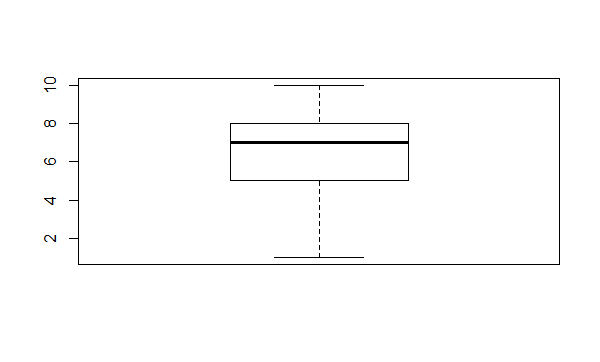
\includegraphics[width=0.7\linewidth]{Rplot2}
				\caption{Boxplot của AttractiveM}
				\label{fig:rplot2}
			\end{figure}
			
			Ta thấy rằng, dữ liệu này khá tốt khi không có ngoại lệ nhưng để chắc chắn thì ta sẽ kiểm định khoảng tin cậy cho trung vị của AttractiveM.
			
			
			Để tính đến sự biến động của $\hat{med}$ theo mẫu dữ liệu $n = 276$ thu thập từ tổng thể, ta thực hiện kiểm định giả thuyết:
			\begin{equation*}
			\begin{cases}
			H_0: med = med_0 = 7.0\\
			H_1: med \neq 7.0
			\end{cases}
			\end{equation*}
			với mức ý nghĩa $\alpha = 0.5\%$
			
			\footnote{Hàm randomization vẫn y như ở câu~\ref{1a}}
			\begin{lstlisting}[language=R]
			# TK can tinh
			stat <- function(data){
				return (median(data, na.rm = TRUE)) # tb mau
			}
			
			> # tham so mac dinh, trung vi mau, muc y nghia
			> (med0 <- 7.0); (med_hat <- stat(sample)); (alpha <- 0.05)
			[1] 7
			[1] 7
			[1] 0.05
			> nullsample <- sample - (med_hat - med0) # Mau du lieu tuong ung voi H0
			> stat(nullsample)
			[1] 7
			 
			> # Lay phan phoi cua randomization
			> rand_dist <- randomization(10000)
			> # Tinh p-value trong kiem dinh hai phia (two-tailed)
			> (p_value <- mean(abs(rand_dist - med0) >= abs(med_hat - med0)))
			[1] 1
			> # Tinh gia tri toi han (critical value) voi muc phan vi 1-alpha/2
			> (crit_val <- quantile(rand_dist, 1 - alpha/2, names = FALSE))
			[1] 7
			> # Kiem tra xem p_value co be hon alpha, neu co thi bac bo H0
			> p_value < alpha; abs(crit_val - med0) < abs(med_hat - med0)
			[1] FALSE
			[1] FALSE
			\end{lstlisting}
			
			Vì $p-value > \alpha$ nên ta không bác bỏ $H_0$. Tương tự, ta có giá trị tới hạn (critical value) $crit\_val > \hat{med}$ nên ta không bác bỏ $H_0$. 
			
			Như vậy, với mức ý nghĩa 5\%, trung vị mức độ quyến rũ của sinh viên nữ trong trường là $7.0$. 
			
	\end{enumerate}
	
	\subsubsection{LikeM (0-10)}
	\begin{enumerate}[label = \alph*)]
		\item Kiểm định cho kì vọng \label{2a}
		
		Giả sử, ta cần khảo sát kì vọng (mean) mức độ thích của nam (0,1,...,10) đối với nữ cho quần thể (population) là toàn bộ sinh viên nam của trường Columbia. Từ tổng thể, ta thu thập được một mẫu dữ liệu ngẫu nhiên (random sample) gồm 276 quan sát. Dựa vào mẫu dữ liệu này, ta kiểm định nghi vấn "Kì vọng mức độ thích của sinh viên nam đối với sinh viên nữ trong trường là 6.6" với mức ý nghĩa (significance level) 5\%.
	
		Gọi $\mu$ là mức độ thích trung bình của sinh viên nam trong trường, $\bar{x}$ là mức độ thích trung bình của sinh nam trong mẫu dữ liệu. Ta có
			$$\bar{x} = \frac{\sum_{i = 1}^{N}x_i}{N} =  6.682$$
		
		Để tính đến sự biến động của $\bar{x}$ theo mẫu dữ liệu $n = 276$ thu thập từ tổng thể, ta thực hiện kiểm định giả thuyết:
		
		\begin{equation*}
		\begin{cases}
		H_0: \mu = \mu_0 = 6.6\\
		H_1: \mu \neq 6.6
		\end{cases}
		\end{equation*}
		với mức ý nghĩa $\alpha = 0.5\%$
		
		\begin{lstlisting}[language=R]
		# TK can tinh
		stat <- function(data){
			return (mean(data, na.rm = TRUE)) # tb mau
		}
		
		randomization <- function(B){
			return (replicate(B, stat(sample(nullsample, n, replace = TRUE))))
		}
		
		> # Mau du lieu ban dau
		> sample <- LikeM
		> # Kich thuoc mau, tham so mac dinh, trung binh mau, muc y nghia
		> (n <- length(sample)); (mu0 <- 6.6); (x_bar <- stat(sample)); (alpha <- 0.05)
		[1] 276
		[1] 6.6
		[1] 6.682482
		[1] 0.05
		> nullsample <- sample - (x_bar - mu0) # Mau du lieu tuong ung voi H0
		> # Check lai mean cua nullsample co bang mu0 chua
		> mean(nullsample, na.rm = TRUE)
		[1] 6.6
		 
		> # Lay phan phoi cua randomization
		> rand_dist <- randomization(10000)
		> # Tinh p-value trong kiem dinh hai phia (two-tailed)
		> (p_value <- mean(abs(rand_dist - mu0) >= abs(x_bar - mu0)))
		[1] 0.4384
		> # Tinh gia tri toi han (critical value) voi muc phan vi 1-alpha/2
		> (crit_val <- quantile(rand_dist, 1 - alpha/2, names = FALSE))
		[1] 6.811291
		> # Kiem tra xem p_value co be hon alpha, neu co thi bac bo H0
		> p_value < alpha; abs(crit_val - mu0) < abs(x_bar - mu0)
		[1] FALSE
		[1] FALSE
		\end{lstlisting}
		
		Vì $p-value > \alpha$ nên ta không bác bỏ $H_0$. Tương tự, ta có giá trị tới hạn (critical value) $crit\_val > \bar{x}$ nên ta không bác bỏ $H_0$. 
		
		Như vậy, với mức ý nghĩa 5\%, kì vọng mức độ thích của sinh viên nam là $6.6$. 
		
		\item Kiểm định cho trung vị (median)
		
		Giả sử cùng tổng thể và mẫu dữ liệu ở câu~\ref{2a} nhưng ta kiểm định cho trung vị mức độ thích của sinh viên nam đối với sinh viên nữ trong trường với mức ý nghĩa (significance level) 5\% thay vì trung bình của mức độ thích. Mặc dù trung bình thường được sử dụng như là con số mô tả trọng tâm của phân phối nhưng nó lại rất nhạy cảm với ngoại lệ (outlier).
		
		Gọi $med$ là median mức độ thích của nam đối với nữ trong trường, $\hat{med}$ là median mức độ thích của nam đối với nữ trong mẫu dữ liệu. Ta có
		$$\hat{med} = 7.000$$
		
		Ta có thể thấy các ngoại lệ qua boxplot sau đây:
		\begin{figure}[H]
			\centering
			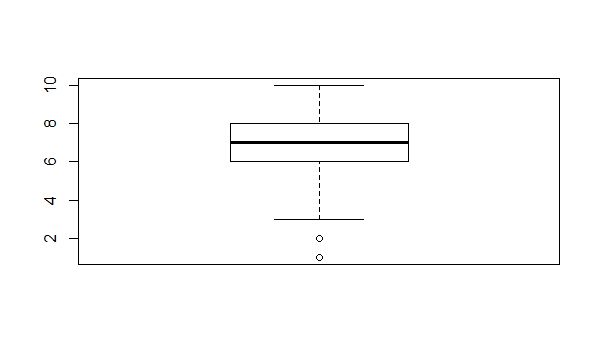
\includegraphics[width=0.7\linewidth]{Rplot1}
			\caption{Boxplot của LikeM}
			\label{fig:rplot1}
		\end{figure}
		
		Ta thấy rằng có một số outliers dưới 3 điểm. Trong những trường hợp như thế này ta có thể dùng trung vị là một thống kê ít bị ảnh hưởng bởi ngoại lệ.
		
		Để tính đến sự biến động của $\hat{med}$ theo mẫu dữ liệu $n = 276$ thu thập từ tổng thể, ta thực hiện kiểm định giả thuyết:
		\begin{equation*}
		\begin{cases}
		H_0: med = med_0 = 7.0\\
		H_1: med \neq 7.0
		\end{cases}
		\end{equation*}
		với mức ý nghĩa $\alpha = 0.5\%$
		
		\footnote{Hàm randomization vẫn y như ở câu~\ref{2a}}
		\begin{lstlisting}[language=R]
		# TK can tinh
		stat <- function(data){
			return (median(data, na.rm = TRUE)) # median
		}
		
		> # tham so mac dinh, trung vi mau, muc y nghia
		> (med0 <- 7.0); (med_hat <- stat(sample)); (alpha <- 0.05)
		[1] 7
		[1] 7
		[1] 0.05
		> nullsample <- sample - (med_hat - med0) # Mau du lieu tuong ung voi H0
		> stat(nullsample)
		[1] 7
		 
		> # Lay phan phoi cua randomization
		> rand_dist <- randomization(10000)
		> # Tinh p-value trong kiem dinh hai phia (two-tailed)
		> (p_value <- mean(abs(rand_dist - med0) >= abs(med_hat - med0)))
		[1] 1
		> # Tinh gia tri toi han (critical value) voi muc phan vi 1-alpha/2
		> (crit_val <- quantile(rand_dist, 1 - alpha/2, names = FALSE))
		[1] 7
		> # Kiem tra xem p_value co be hon alpha, neu co thi bac bo H0
		> p_value < alpha; abs(crit_val - med0) < abs(med_hat - med0)
		[1] FALSE
		[1] FALSE
		\end{lstlisting}
		
		Vì $p-value > \alpha$ nên ta không bác bỏ $H_0$. Tương tự, ta có giá trị tới hạn (critical value) $crit\_val > \hat{med}$ nên ta không bác bỏ $H_0$. 
		
		Như vậy, với mức ý nghĩa 5\%, trung vị mức độ thích của sinh viên nam đối với sinh viên nữ trong trường là $7.0$. 
	\end{enumerate}
	
	\subsubsection{SincereM (0-10)}
	\begin{enumerate}[label = \alph*)]
		\item Kiểm định cho kì vọng \label{3a}
		
		Giả sử, ta cần khảo sát kì vọng (mean) mức độ chân thành (0,1,...,10) của nữ cho quần thể (population) là toàn bộ sinh viên nữ của trường Columbia. Từ tổng thể, ta thu thập được một mẫu dữ liệu ngẫu nhiên (random sample) gồm 276 quan sát. Dựa vào mẫu dữ liệu này, ta kiểm định nghi vấn "Kì vọng mức độ chân thành của sinh viên nữ trong trường là 7.8" với mức ý nghĩa (significance level) 5\%.
		
		Gọi $\mu$ là mức độ chân thành trung bình của sinh viên nữ trong trường, $\bar{x}$ là mức độ chân thành trung bình của sinh nữ trong mẫu dữ liệu. Ta có
		$$\bar{x} = \frac{\sum_{i = 1}^{N}x_i}{N} =  7.856$$
		
		Để tính đến sự biến động của $\bar{x}$ theo mẫu dữ liệu $n = 276$ thu thập từ tổng thể, ta thực hiện kiểm định giả thuyết:
		
		\begin{equation*}
		\begin{cases}
		H_0: \mu = \mu_0 = 7.8\\
		H_1: \mu \neq 7.8
		\end{cases}
		\end{equation*}
		với mức ý nghĩa $\alpha = 0.5\%$
		
		\begin{lstlisting}[language=R]
		# TK can tinh
		stat <- function(data){
			return (mean(data, na.rm = TRUE)) # tb mau
		}
		
		randomization <- function(B){
			return (replicate(B, stat(sample(nullsample, n, replace = TRUE))))
		}
		
		> # Mau du lieu ban dau
		> sample <- SincereM
		> # Kich thuoc mau, tham so mac dinh, trung binh mau, muc y nghia
		> (n <- length(sample)); (mu0 <- 7.8); (x_bar <- stat(sample)); (alpha <- 0.05)
		[1] 276
		[1] 7.8
		[1] 7.856089
		[1] 0.05
		> nullsample <- sample - (x_bar - mu0) # Mau du lieu tuong ung voi H0
		> # Check lai mean cua nullsample co bang mu0 chua
		> mean(nullsample, na.rm = TRUE)
		[1] 7.8
		 
		> # Lay phan phoi cua randomization
		> rand_dist <- randomization(10000)
		> # Tinh p-value trong kiem dinh hai phia (two-tailed)
		> (p_value <- mean(abs(rand_dist - mu0) >= abs(x_bar - mu0)))
		[1] 0.5422
		> # Tinh gia tri toi han (critical value) voi muc phan vi 1-alpha/2
		> (crit_val <- quantile(rand_dist, 1 - alpha/2, names = FALSE))
		[1] 7.976758
		> # Kiem tra xem p_value co be hon alpha, neu co thi bac bo H0
		> p_value < alpha; abs(crit_val - mu0) < abs(x_bar - mu0)
		[1] FALSE
		[1] FALSE
		\end{lstlisting}
		
		Vì $p-value > \alpha$ nên ta không bác bỏ $H_0$. Tương tự, ta có giá trị tới hạn (critical value) $crit\_val > \bar{x}$ nên ta không bác bỏ $H_0$. 
		
		Như vậy, với mức ý nghĩa 5\%, kì vọng mức độ chân thành của sinh viên nữ là $7.8$.
	
		\item Kiểm định cho trung vị (median)
		
		Giả sử cùng tổng thể và mẫu dữ liệu ở câu~\ref{3a} nhưng ta kiểm định cho trung vị mức độ chân thành của sinh viên nữ trong trường với mức ý nghĩa (significance level) 5\% thay vì trung bình của mức độ chân thành. Mặc dù trung bình thường được sử dụng như là con số mô tả trọng tâm của phân phối nhưng nó lại rất nhạy cảm với ngoại lệ (outlier).
		
		Gọi $med$ là median mức độ chân thành của nữ trong trường, $\hat{med}$ là median mức độ chân thành trong mẫu dữ liệu. Ta có
		$$\hat{med} = 8.000$$
		
		Ta có thể thấy các ngoại lệ qua boxplot sau đây:
		\begin{figure}[H]
			\centering
			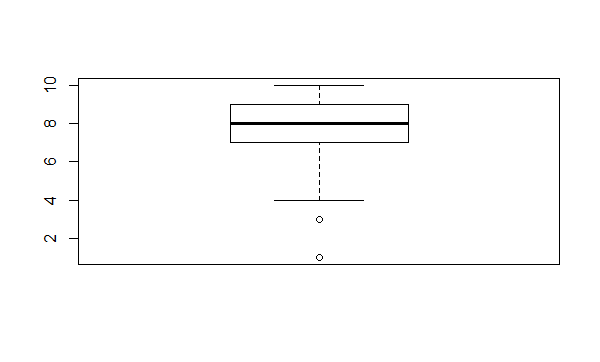
\includegraphics[width=0.7\linewidth]{Rplot3}
			\caption{Boxplot của LikeM}
			\label{fig:rplot3}
		\end{figure}
	
		Ta thấy rằng có một số outliers dưới 4 điểm. Trong những trường hợp như thế này ta có thể dùng trung vị là một thống kê ít bị ảnh hưởng bởi ngoại lệ.
		
		Để tính đến sự biến động của $\hat{med}$ theo mẫu dữ liệu $n = 276$ thu thập từ tổng thể, ta thực hiện kiểm định giả thuyết:
		\begin{equation*}
		\begin{cases}
		H_0: med = med_0 = 8.0\\
		H_1: med \neq 8.0
		\end{cases}
		\end{equation*}
		với mức ý nghĩa $\alpha = 0.5\%$
		
		\footnote{Hàm randomization vẫn y như ở câu~\ref{3a}}
		\begin{lstlisting}[language=R]
		# TK can tinh
		stat <- function(data){
			return (median(data, na.rm = TRUE)) # trung vi
		}
		
		> # tham so mac dinh, trung vi mau, muc y nghia
		> (med0 <- 8.0); (med_hat <- stat(sample)); (alpha <- 0.05)
		[1] 8
		[1] 8
		[1] 0.05
		> nullsample <- sample - (med_hat - med0) # Mau du lieu tuong ung voi H0
		> stat(nullsample)
		[1] 8
		 
		> # Lay phan phoi cua randomization
		> rand_dist <- randomization(10000)
		> # Tinh p-value trong kiem dinh hai phia (two-tailed)
		> (p_value <- mean(abs(rand_dist - med0) >= abs(med_hat - med0)))
		[1] 1
		> # Tinh gia tri toi han (critical value) voi muc phan vi 1-alpha/2
		> (crit_val <- quantile(rand_dist, 1 - alpha/2, names = FALSE))
		[1] 8
		> # Kiem tra xem p_value co be hon alpha, neu co thi bac bo H0
		> p_value < alpha; abs(crit_val - med0) < abs(med_hat - med0)
		[1] FALSE
		[1] FALSE
		\end{lstlisting}
		
		Vì $p-value > \alpha$ nên ta không bác bỏ $H_0$. Tương tự, ta có giá trị tới hạn (critical value) $crit\_val > \hat{med}$ nên ta không bác bỏ $H_0$. 
		
		Như vậy, với mức ý nghĩa 5\%, trung vị mức độ chân thành của sinh viên nữ trong trường là $8.0$. 
	\end{enumerate}
	
	\section{Khảo sát cặp biến}
	\subsection{Biến định tính vs biến định tính}
	Chọn 2 biến định tính: DecisionMale (Yes/No) và RaceF (Asian, Black, Caucasian, Latino, Other)
	
	Khảo sát 2 biến định tính DecisionMale và RaceF
	
	\begin{lstlisting}[language=R]
	# 2 bien dinh tinh
	tab1 = table(DecisionMale, RaceF)
	# Them margin
	addmargins(tab1)
	>
	 RaceF
	DecisionMale     Asian Black Caucasian Latino Other Sum
	No    2    32     7        72      7    10 130
	Yes   2    38     8        76     16     6 146
	Sum   4    70    15       148     23    16 276
	
	# 2-way table
	# Ti le chung toc nu (Asian, Black, ...) nhan phan hoi
	prop.table(tab1, margin = 1)
	>
	            RaceF
	DecisionMale                 Asian      Black  Caucasian     Latino      Other
	No  0.01538462 0.24615385 0.05384615 0.55384615 0.05384615 0.07692308
	Yes 0.01369863 0.26027397 0.05479452 0.52054795 0.10958904 0.04109589
	
	barplot(tab1, legend = TRUE)
	\end{lstlisting}
	\begin{figure}[H]
		\centering
		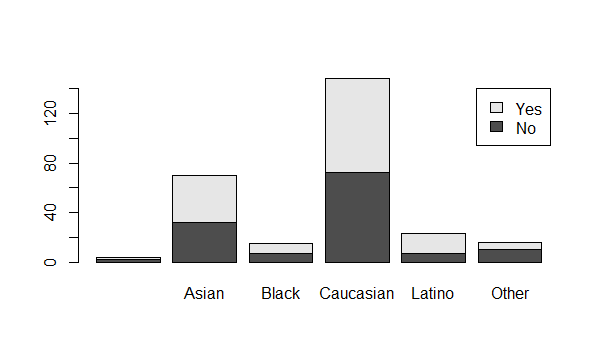
\includegraphics[width=0.7\linewidth]{Rplot4}
		\caption{Segmented barchart của DecisionMale và RaceF}
		\label{fig:rplot4}
	\end{figure}
	

	
	\subsubsection{Kiểm định cho tỉ lệ khác biệt giữa nữ da trắng nhận phản hồi "Yes" và "No"}
		Giả sử, ta cần khảo sát tỉ lệ khác biệt giữa nữ da trắng được nam phản hồi (Yes/No) cho quần thể (population) là toàn bộ sinh viên nữ của trường Columbia bằng cách gom nhóm các dân tộc nữ khác còn lại thành 1 cụm.\\
		
		Ta chỉ phân tích giữa tỉ lệ nữ da trắng và nhóm còn lại. Từ tổng thể, ta thu thập được một mẫu dữ liệu ngẫu nhiên (random sample) gồm 276 quan sát trong đó có 148 nữ da trắng (gồm 76 phản hồi "Yes", 72 phản hồi "No") và 128 dân tộc khác (gồm 70 phản hồi "Yes" và 58 phản hồi "No").\\
		
		Dựa vào mẫu dữ liệu này, ta kiểm định nghi vấn "Tỉ lệ nữ da trắng nhận phản hồi Yes nhiều hơn phản hồi No" với mức ý nghĩa (significance level) 5\%.\\
		
		Gọi $p_{Yes}$ là tỉ lệ nữ da trắng nhận phản hồi "Yes" và $p_{No}$ là tỉ lệ nữ da trắng nhận phản hồi "No" trong trường. Từ đây, suy ra tỉ lệ khác biệt giữa phản hồi Yes và phản hồi No trong trường là $\Delta p$: 
		$$\Delta p = p_{Yes} - p_{No}$$
		
		Gọi $\hat{p}_{Yes}$ là tỉ lệ nữ da trắng nhận phản hồi "Yes" và $\hat{p}_{No}$ là tỉ lệ nữ da trắng nhận phản hồi "No" trong mẫu dữ liệu. Từ đây, suy ra tỉ lệ khác biệt giữa phản hồi Yes và phan hồi No trong mẫu dữ liệu là $\Delta\hat{p}$:
		$$\Delta\hat{p} = \hat{p}_{Yes} - \hat{p}_{No} = 0.01449275$$
		
		Để tính đến sự biến động của $\Delta\hat{p}$ theo mẫu dữ liệu $n = 276$ thu thập từ tổng thể, ta thực hiện kiểm định giả thuyết:
		
		\begin{equation*}
		\begin{cases}
		H_0: \Delta p = \Delta p_0 = 0\\
		H_1: \Delta p > 0
		\end{cases}
		\end{equation*}
		với mức ý nghĩa $\alpha = 0.5\%$
		
		\begin{lstlisting}[language=R]
		stat <- function(data){
			return (mean(data$DecisionMale == 'Yes' & data$RaceF == 'Caucasian') - mean(data$DecisionMale == 'No' & data$RaceF == 'Caucasian')) # Ti le khac biet
		}
		
		randomization <- function(B){
			return (replicate(B, stat(sample(nullsample, n, replace = TRUE))))
		}
		
		> # Mau du lieu ban dau
		> sample <- data.frame(DecisionMale, RaceF)
		> # tham so mac dinh, ti le mau, muc y nghia
		> (p0 <- 0.5); (p_hat <- stat(sample)); (alpha <- 0.05)
		[1] 0.5
		[1] 0.01449275
		[1] 0.05
		> # Kich thuoc mau
		> (n <- nrow(sample))
		[1] 276
		> nullsample <- data.frame("DecisionMale" = c(rep("Yes", n/2), rep("No", n/2)), "RaceF" = rep("Caucasian", n)) # Mau du lieu tuong ung voi H0 
		
		> # Lay phan phoi cua randomization
		> rand_dist <- randomization(10000)
		> # Tinh p-value trong kiem dinh mot phia (one-tailed)
		> (p_value <- mean(rand_dist >= p_hat))
		[1] 0.4285
		> # Tinh gia tri toi han (critical value) voi muc phan vi 1-alpha
		> (crit_val <- quantile(rand_dist, 1 - alpha, names = FALSE))
		[1] 0.1014493
		> # Kiem tra xem p_value co be hon alpha, neu co thi bac bo H0
		> p_value < alpha; crit_val < p_hat
		[1] FALSE
		[1] FALSE
		\end{lstlisting}
	
		Vì $p-value > \alpha$ nên ta không bác bỏ $H_0$. Tương tự, ta có giá trị tới hạn (critical value) $crit\_val > \Delta\hat{p}$ nên ta không bác bỏ $H_0$. 
	
		Như vậy, với mức ý nghĩa 5\%, tỉ lệ nữ da trắng nhận phản hồi "Yes" bằng với phản hồi "No".
		
		\subsubsection{Kiểm định cho tỉ lệ khác biệt giữa nữ châu Á nhận phản hồi "Yes"/"No"}
		
			Giả sử, ta cần khảo sát tỉ lệ khác biệt giữa nữ châu Á được nam phản hồi (Yes/No) cho quần thể (population) là toàn bộ sinh viên nữ của trường Columbia bằng cách gom nhóm các dân tộc nữ khác còn lại thành 1 cụm.\\
			
			Ta chỉ phân tích giữa tỉ lệ nữ châu Á và nhóm còn lại. Từ tổng thể, ta thu thập được một mẫu dữ liệu ngẫu nhiên (random sample) gồm 276 quan sát trong đó có 70 nữ châu Á (gồm 32 phản hồi "Yes", 32 phản hồi "No") và 206 dân tộc khác (gồm 108 phản hồi "Yes" và 98 phản hồi "No").\\
			
			Dựa vào mẫu dữ liệu này, ta kiểm định nghi vấn "Tỉ lệ nữ châu Á nhận phản hồi Yes bằng với phản hồi No" với mức ý nghĩa (significance level) 5\%.\\
		
			Gọi $p_{Yes}$ là tỉ lệ nữ châu Á nhận phản hồi "Yes" và $p_{No}$ là tỉ lệ nữ châu Á nhận phản hồi "No" trong trường. Từ đây, suy ra tỉ lệ khác biệt giữa phản hồi Yes và phản hồi No trong trường là $\Delta p$: 
			$$\Delta p = p_{Yes} - p_{No}$$
			
			Gọi $\hat{p}_{Yes}$ là tỉ lệ nữ châu Á nhận phản hồi "Yes" và $\hat{p}_{No}$ là tỉ lệ nữ châu Á nhận phản hồi "No" trong mẫu dữ liệu. Từ đây, suy ra tỉ lệ khác biệt giữa phản hồi Yes và phản hồi No trong mẫu dữ liệu là $\Delta\hat{p}$:
			$$\Delta\hat{p} = \hat{p}_{Yes} - \hat{p}_{No} = 0.02173913$$
			
			Để tính đến sự biến động của $\Delta\hat{p}$ theo mẫu dữ liệu $n = 276$ thu thập từ tổng thể, ta thực hiện kiểm định giả thuyết:
			
			\begin{equation*}
			\begin{cases}
			H_0: \Delta p = \Delta p_0 = 0\\
			H_1: \Delta p \neq 0
			\end{cases}
			\end{equation*}
			với mức ý nghĩa $\alpha = 0.5\%$
			
			\begin{lstlisting}[language=R]
			# TK can tinh
			stat <- function(data){
				return (mean(data$DecisionMale == 'Yes' & data$RaceF == 'Asian') - mean(data$DecisionMale == 'No' & data$RaceF == 'Asian')) # Ti le khac biet
			}
			
			randomization <- function(B){
				return (replicate(B, stat(sample(nullsample, n, replace = TRUE))))
			}
			
			> # tham so mac dinh, ti le mau, muc y nghia
			> (p0 <- 0); (p_hat <- stat(sample)); (alpha <- 0.05)
			[1] 0
			[1] 0.02173913
			[1] 0.05
			> # Kich thuoc mau
			> (n <- nrow(sample))
			[1] 276
			> nullsample <- data.frame("DecisionMale" = c(rep("Yes", n/2), rep("No", n/2)), "RaceF" = rep("Asian", n)) # Mau du lieu tuong ung voi H0
			
			> # Lay phan phoi cua randomization
			> rand_dist <- randomization(10000)
			> # Tinh p-value trong kiem dinh mot phia (one-tailed)
			> (p_value <- mean(abs(rand_dist - p0) >= abs(p_hat - p0)))
			[1] 0.7658
			> # Tinh gia tri toi han (critical value) voi muc phan vi 1-alpha/2
			> (crit_val <- quantile(rand_dist, 1 - alpha/2, names = FALSE))
			[1] 0.115942
			> # Kiem tra xem p_value co be hon alpha, neu co thi bac bo H0
			> p_value < alpha; crit_val < p_hat
			[1] FALSE
			[1] FALSE
			\end{lstlisting}
			
			Vì $p-value > \alpha$ nên ta không bác bỏ $H_0$. Tương tự, ta có giá trị tới hạn (critical value) $crit\_val > \Delta\hat{p}$ nên ta không bác bỏ $H_0$.
			
			Như vậy, với mức ý nghĩa 5\%, tỉ lệ nữ châu Á nhận phản hồi "Yes" bằng với phản hồi "No".
		
		
	\subsection{Biến định tính và biến định lượng}
	Chon 1 biến định tính và 1 biến định lượng: ̣DecisionMale (yes/no), AttractiveM (1-10)
	
	\begin{lstlisting}[language = R]
	# Tinh favorite statistics
	> favstats(AttractiveM ~ DecisionMale)
	DecisionMale min Q1 median Q3 max     mean       sd   n missing
	1           No   1  5      5  6  10 5.641732 1.694877 127       3
	2          Yes   5  7      8  8  10 7.595890 1.357375 146       0
	
	# Ve boxplot
	boxplot(AttractiveM ~ DecisionMale, xlab = "DecisionMale", ylab = "AttractiveM")
	\end{lstlisting}
	\begin{figure}[H]
		\centering
		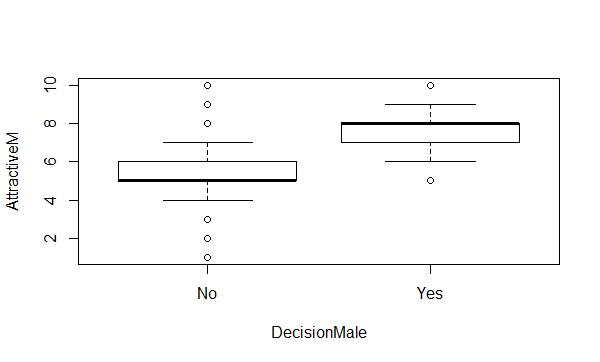
\includegraphics[width=0.7\linewidth]{Rplot5}
		\caption{Side-by-side boxplots}
		\label{fig:rplot5}
	\end{figure}
	
	\subsubsection{Kiểm định cho độ chênh lệch kì vọng giữa mức độ hấp dẫn của nữ trong phản hồi "Yes" và mức độ hấp dẫn của nữ trong phản hồi "No"}
	
	Giả sử, ta cần khảo sát kì vọng chênh lệch giữa mức độ hấp dẫn của nữ trong phản hồi "Yes" và trong phản hồi "No" cho quần thể (population) là toàn bộ sinh viên nữ của trường Columbia.\\
	
	Từ tổng thể, ta thu thập được một mẫu dữ liệu ngẫu nhiên (random sample) gồm 276 quan sát. Dựa vào mẫu dữ liệu này, ta kiểm định nghi vấn "Kì vọng mức độ hấp dẫn của nữ trong phản hồi Yes sẽ cao hơn trong phản hồi No" với mức ý nghĩa (significance level) 5\%.\\
	
	Gọi $\mu_{AttractiveM|Yes}$ là kì vọng mức độ hấp dẫn của nữ nhận phản hồi "Yes" và $\mu_{AttractiveM|No}$ là kì vọng mức độ hấp dẫn của nữa nhận phản hồi "No" trong trường. Từ đây, suy ra độ chênh lệch kì vọng giữa phản hồi Yes và phản hồi No trong trường là $\Delta\mu$:
	$$\Delta\mu = \mu_{AttractiveM|Yes} - \mu_{AttractiveM|No}$$
	
	Gọi $\bar{x}_{AttractiveM|Yes}$ là mức độ hấp dẫn trung bình của nữ nhận phản hồi "Yes" và $\bar{x}_{AttractiveM|No}$ là mức độ hấp dẫn trung bình của nữ nhận phản hồi "No" trong mẫu dữ liệu. Từ đây, suy ra độ chênh lệch kì vọng giữa phản hồi Yes và phản hồi No trong mẫu dữ liệu là $\Delta\bar{x}$:
	$$\Delta\bar{x} = \bar{x}_{AttractiveM|Yes} - \bar{x}_{AttractiveM|No} = 1.954158$$
	
	Để tính đến sự biến động của $\Delta\bar{x}$ theo mẫu dữ liệu $n = 276$ thu thập từ tổng thể, ta thực hiện kiểm định giả thuyết:
	
	\begin{equation*}
	\begin{cases}
	H_0: \Delta\mu = \Delta\mu_0 = 0\\
	H_1: \Delta\mu > 0
	\end{cases}
	\end{equation*}
	với mức ý nghĩa $\alpha = 0.5\%$
	
	\begin{lstlisting}[language=R]
	# TK can tinh
	diffmean <- function(data1, data2) {
		# Lay index
		index <- 1:(n1+n2) %in% sample(1:(n1+n2), n1)
		# random sample cua yes
		rand_sample1 <- c(data1, data2)[index]
		# random sample cua no
		rand_sample2 <- c(data1, data2)[!index]
		return(mean(rand_sample1, na.rm = TRUE)-mean(rand_sample2, na.rm = TRUE))
	}
	
	randomization <- function(B){
		return (replicate(B, diffmean(sample1, sample2)))
	}
	
	> # Sample
	> sample1 <- subset(SpeedDating, DecisionMale=='Yes', select=c(AttractiveM))[[1]]; 
	> sample2 <- subset(SpeedDating, DecisionMale=='No', select=c(AttractiveM))[[1]];
	> # Kich thuoc mau
	> n1 <- length(sample1); n2 <- length(sample2); n1; n2
	[1] 146
	[1] 130
	 
	> # tb mau 1, tb mau 2 va diff mean cua mau 1 va 2
	> (x_1 <- mean(sample1, na.rm = TRUE)); (x_2 <- mean(sample2, na.rm = TRUE)); (diff_x <- x_1 - x_2)
	[1] 7.59589
	[1] 5.641732
	[1] 1.954158
	> # tham so mac dinh, muc y nghia
	> (diff_mu0 <- 0); (alpha <- 0.05)
	[1] 0
	[1] 0.05
	
	> # Lay phan phoi cua randomization
	> rand_dist <- randomization(10000); hist(rand_dist)
	> # Tinh p-value trong kiem dinh mot phia (one-tailed)
	> (p_value <- mean(rand_dist >= diff_x))
	[1] 0
	> # Tinh gia tri toi han (critical value) voi muc phan vi 1-alpha
	> (crit_val <- quantile(rand_dist, 1 - alpha, names = FALSE))
	[1] 0.3517241
	> # Kiem tra xem p_value co be hon alpha, neu co thi bac bo H0
	> p_value < alpha; crit_val < diff_x
	[1] TRUE
	[1] TRUE
	\end{lstlisting}
	
	Vì $p-value < \alpha$ nên ta bác bỏ $H_0$, chấp nhận $H_1$. Tương tự, ta có giá trị tới hạn (critical value) $crit\_val < \Delta\bar{x}$ nên ta bác bỏ $H_0$, chấp nhận $H_1$. 
	
	Như vậy, với mức ý nghĩa 5\%, kì vọng mức độ quyến rũ trong phản hồi "Yes" cao hơn phản hồi "No".

	\subsubsection{Kiểm định cho độ chênh lệch trung vị (median) giữa mức độ hấp dẫn của nữ trong phản hồi "Yes" và mức độ hấp dẫn của nữ trong phản hồi "No"}
	
	Giả sử cùng tổng thể và mẫu dữ liệu ở câu trên nhưng ta muốn xây dựng khoảng tin cậy 95\% cho
	trung vị (median) thay vì trung bình của mức độ hấp dẫn trong phản hồi "Yes"/"No". Mặc dù trung bình thường được sử dụng như là con số mô tả trọng tâm của phân phối nhưng nó lại rất nhạy cảm với ngoại lệ (outlier).\\
	
	Ta có thể thấy trong \ref{fig:rplot5} ở mỗi phản hồi "Yes" và "No" đều có các outlier xuất hiện đặc biết nhất là ở phản hồi "No", có những điểm số bất thường như 8, 9, 10 vẫn nằm trong phản hồi "No".\\
	
	Gọi $med_{AttractiveM|Yes}$ là median mức độ hấp của quyến rũ trong phản hồi "Yes" và $med_{AttractiveM|No}$ là median mức độ quyến rũ của nữ trong phản hồi "No" của trường. Từ đây, suy ra độ chênh lệch trung vị giữa phản hồi Yes và phản hồi No trong trường là $\Delta med$:
	$$\Delta med = med_{AttractiveM|Yes} - med_{AttractiveM|No}$$
	
	Gọi $\hat{med}_{AttractiveM|Yes}$ là median mức độ hấp dẫn của nữ trong phản hồi "Yes" và  $\hat{med}_{AttractiveM|No}$ là median mức độ hấp dẫn của nữ trong phản hồi "No" của mẫu dữ liệu. Từ đây, suy ra độ chênh lệch trung vị giữa phản hồi Yes và phản hồi No trong mẫu dữ liệu là $\Delta\hat{med}$:
	$$\Delta\hat{med} = \hat{med}_{AttractiveM|Yes} - \hat{med}_{AttractiveM|No} = 3$$
	
	Để tính đến sự biến động của $\Delta\hat{med}$ theo mẫu dữ liệu $n = 276$ thu thập từ tổng thể, ta thực hiện kiểm định giả thuyết:
	
	\begin{equation*}
	\begin{cases}
	H_0: \Delta med = \Delta med_0 = 0\\
	H_1: \Delta med > 0
	\end{cases}
	\end{equation*}
	với mức ý nghĩa $\alpha = 0.5\%$
	
	Ta có thể thấy rằng, median kháng nhiễu tốt hơn so với mean dựa vào số liệu thống kê trên.\\
	
	\begin{lstlisting}[language=R]
	# TK can tinh
	diffmed <- function(data1, data2) {
		# Lay index
		index <- 1:(n1+n2) %in% sample(1:(n1+n2), n1)
		# random sample cua yes
		rand_sample1 <- c(data1, data2)[index];
		# random sample cua no
		rand_sample2 <- c(data1, data2)[!index];
		return(median(rand_sample1, na.rm = TRUE)-median(rand_sample2, na.rm = TRUE))
	}
	
	randomization <- function(B){
		return (replicate(B, diffmed(sample1, sample2)))
	}
	
	> # Sample
	> sample1 <- subset(SpeedDating, DecisionMale=='Yes', select=c(AttractiveM))[[1]]; 
	> sample2 <- subset(SpeedDating, DecisionMale=='No', select=c(AttractiveM))[[1]];
	> # Kich thuoc mau
	> n1 <- length(sample1); n2 <- length(sample2); n1; n2
	[1] 146
	[1] 130
	
	> # med mau 1, med mau 2 va diff med cua mau 1 va 2
	> (med_1 <- median(sample1, na.rm = TRUE)); (med_2 <- median(sample2, na.rm = TRUE)); (diff_med <- med_1 - med_2)
	[1] 8
	[1] 5
	[1] 3
	> # tham so mac dinh, muc y nghia
	> (diff_med0 <- 0); (alpha <- 0.05)
	[1] 0
	[1] 0.05
	
	> # Lay phan phoi cua randomization
	> rand_dist <- randomization(10000); hist(rand_dist)
	> # Tinh p-value trong kiem dinh mot phia (one-tailed)
	> (p_value <- mean(rand_dist >= diff_med))
	[1] 0
	> # Tinh gia tri toi han (critical value) voi muc phan vi 1-alpha
	> (crit_val <- quantile(rand_dist, 1 - alpha, names = FALSE))
	[1] 1
	> # Kiem tra xem p_value co be hon alpha, neu co thi bac bo H0
	> p_value < alpha; crit_val < diff_med
	[1] TRUE
	[1] TRUE
	\end{lstlisting}
	
	\begin{figure}[H]
		\centering
		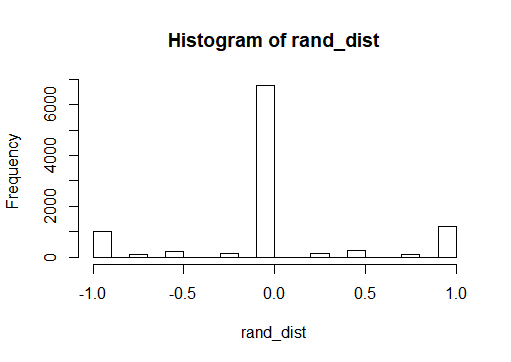
\includegraphics[width=0.7\linewidth]{hist}
		\caption{Histogram của randomization distribution}
		\label{fig:hist}
	\end{figure}
	
	Vì $p-value < \alpha$ nên ta bác bỏ $H_0$, chấp nhận $H_1$. Tương tự, ta có giá trị tới hạn (critical value) $crit\_val < \Delta\hat{med}$ nên ta bác bỏ $H_0$, chấp nhận $H_1$. 
	
	Như vậy, với mức ý nghĩa 5\%, trung vị mức độ quyến rũ trong phản hồi "Yes" cao hơn phản hồi "No".
	
	\subsection{Biến định lượng và biến định lượng}
	Chọn 2 biến định lượng: AttractiveM (1-10) và LikeM (1-10)
	\begin{lstlisting}[language=R]
	# Correlation of 2 quantative variables: AttractiveM and LikeM
	> cor(AttractiveM, LikeM, use = "complete.obs") # Avoid missing values
	[1] 0.7240187
	
	# Fit regression line
	lmInfo <- lm(LikeM~AttractiveM)
	> summary(lmInfo) # get more info
	Call:
	lm(formula = LikeM ~ AttractiveM)
	
	Residuals:
	Min      1Q  Median      3Q     Max 
	-4.6225 -0.6225  0.0914  0.8054  3.6611 
	
	Coefficients:
	Estimate Std. Error t value Pr(>|t|)    
	(Intercept)  1.91100    0.28616   6.678 1.37e-10 ***
	AttractiveM  0.71394    0.04132  17.279  < 2e-16 ***
	---
	Signif. codes:  0 ‘***’ 0.001 ‘**’ 0.01 ‘*’ 0.05 ‘.’ 0.1 ‘ ’ 1
	
	Residual standard error: 1.232 on 271 degrees of freedom
	(3 observations deleted due to missingness)
	Multiple R-squared:  0.5242,	Adjusted R-squared:  0.5224 
	F-statistic: 298.6 on 1 and 271 DF,  p-value: < 2.2e-16
	
	# Graphical display: scatterplot
	plot(AttractiveM, LikeM, main = "Scatter plot example", pch=19)
	# Add fit lines
	abline(lm(LikeM~AttractiveM), col="red") # regression line (y~x)
	
	plot(lmInfo$residuals, pch = 16, col = "red") #Plot residual de xem du lieu co phan bo ngau nhieu khong?
	\end{lstlisting}
	
	\begin{figure}[H]
		\centering
		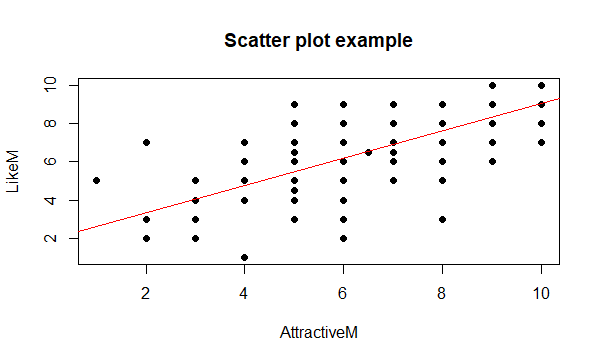
\includegraphics[width=0.7\linewidth]{Rplot6}
		\caption{Scatterplot của 2 biến định lượng và có linear regression line}
		\label{fig:rplot6}
	\end{figure}
	
	\begin{figure}[H]
		\centering
		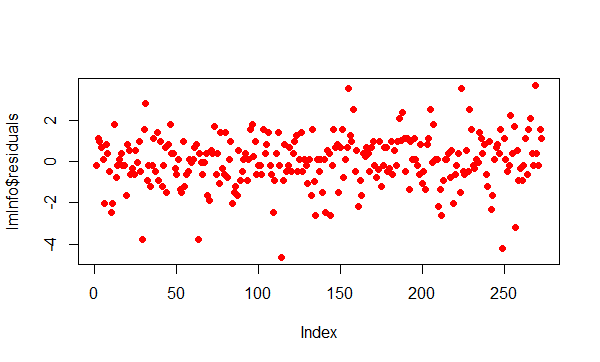
\includegraphics[width=0.7\linewidth]{Rplot7}
		\caption{Residuals plot}
		\label{fig:rplot7}
	\end{figure}
	
	\textbf{Nhận xét:}
	\begin{itemize}
		\item Nhìn vào Residuals, ta thấy rằng độ lệch giữa giá trị dự đoán và giá trị quan sát vẫn còn chệnh lệch khá nhiều.
		\item Tiếp theo, để đánh giá model này có tốt hay không thì ta cần nhìn vào $R^2 = 0.5242$ thì ta thấy nó gần 0.5. Điều này có thể tạm chấp nhận là model này khá tốt.
		\item Nhưng đến đây ta chưa thể vội kết luận rằng model này tốt. Do đó, ta cần plot residuals để xem phân bố của chúng có ngẫu nhiên không. Nếu không ngẫu nhiên mà có thể là có 1 hidden pattern mà model chưa xét tới. Điều này sẽ ảnh hưởng đến khả năng dự đoán khi mà dữ liệu tăng.
		\item Nhìn vào hình \ref{fig:rplot7}, ta đã có thể yên tâm kết luận rằng model này là tốt vì các residuals phân bố ngẫu nhiên (không có hidden pattern như: curve,...)
	\end{itemize}
	
	\subsubsection{Kiểm định cho hệ số tương quan giữa AttractiveM và LikeM}
	Giả sử, ta cần khảo sát hệ số tương quan (correlation coefficient) giữa mức độ hấp dẫn và mức độ thích của nam giới đánh giá cho nữ (AttractiveM và LikeM) cho quần thể (population) là toàn bộ sinh viên nữ của trường Columbia.\\
	
	Từ tổng thể, ta thu thập được một mẫu dữ liệu ngẫu nhiên (random sample) gồm 276 quan sát. Dựa vào mẫu dữ liệu này, ta kiểm định nghi vấn "hệ số tương quan giữa AttractiveM và LikeM lớn hơn 0.5" với mức ý nghĩa (significance level) 5\%.\\
	
	Gọi $\rho$ là hệ số tương quan giữa AttractiveM và LikeM của sinh viên nữ trong trường và $r$ là hệ số tương quan giữa AttractiveM và LikeM của sinh viên nữ trong mẫu dữ liệu. Từ các thống kê tính được bằng R, ta có: $$r = 0.7240187$$
	
	Để tính đến sự biến động của $r$ theo mẫu dữ liệu $n = 276$ thu thập từ tổng thể, ta thực hiện kiểm định giả thuyết:
	
	\begin{equation*}
	\begin{cases}
	H_0: \rho = \rho_0 = 0.5\\
	H_1: \rho > 0.5
	\end{cases}
	\end{equation*}
	với mức ý nghĩa $\alpha = 0.5\%$
	
	\begin{lstlisting}[language=R]
	library("ecodist") # Generate data.frame with specific correlation
	
	#TK can tinh
	stat <- function(data){
		#Tinh correlation
		return (cor(data$AttractiveM, data$LikeM, use = "complete.obs")) # Avoid missing values
	}
	
	randomization <- function(B){
		return (replicate(B, stat(sample(nullsample, n, replace = TRUE))))
	}
	
	> # Sample
	> sample <- data.frame(AttractiveM, LikeM)
	> # Kich thuoc mau
	> (n <- nrow(sample))
	[1] 276
	 
	> # tham so mac dinh, correlation tren mau, muc y nghia
	> (cor0 <- 0.5); (cor_hat <- stat(sample)); (alpha <- 0.05)
	[1] 0.5
	[1] 0.7240187
	[1] 0.05
	> nullsample <- corgen(len = n, r = 0.5, epsilon = 0.01) # Mau tuong thich voi H0
	> #rename column
	> names(nullsample)[1] = "AttractiveM"
	> names(nullsample)[2] = "LikeM"
	> stat(nullsample)
	[1] 0.5089513
	 
	> # Lay phan phoi cua randomization
	> rand_dist <- randomization(10000)
	> # Tinh p-value trong kiem dinh mot phia (one-tailed)
	> (p_value <- mean(rand_dist >= cor_hat))
	[1] 0
	> # Tinh gia tri toi han (critical value) voi muc phan vi 1-alpha
	> (crit_val <- quantile(rand_dist, 1 - alpha, names = FALSE))
	[1] 0.5089513
	> # Kiem tra xem p_value co be hon alpha, neu co thi bac bo H0
	> p_value < alpha; crit_val < cor_hat
	[1] TRUE
	[1] TRUE
	\end{lstlisting}
	
	Vì $p-value < \alpha$ nên ta bác bỏ $H_0$, chấp nhận $H_1$. Tương tự, ta có giá trị tới hạn (critical value) $crit\_val < r$ nên ta bác bỏ $H_0$, chấp nhận $H_1$. 
	
	Như vậy, với mức ý nghĩa 5\%, Hệ số tương quan giữa AttractiveM và LikeM lớn hơn 0.5.\\
		
	\textbf{Nhận xét:}
	\begin{itemize}
		\item Ta có thể thấy rằng đây là 1 liên kết dương mạnh. (do $\rho > 0.5$) 
		\item Điều này có nghĩa là mức độ hấp dẫn của nữ AttractiveM tăng thì mức độ thích của nam dành cho nữ LikeM cũng tăng.
	\end{itemize}
	
	\subsubsection{Kiểm định cho hệ số hồi qui $\beta$ (regression slope) của regression line}
	
	Giả sử, ta cần khảo sát hệ số hồi qui của best-fit line: $\beta$ (slope) giữa mức độ hấp dẫn và mức độ thích của nam giới đánh giá cho nữ (AttractiveM và LikeM) cho quần thể (population) là toàn bộ sinh viên nữ của trường Columbia.\\
	
	Từ tổng thể, ta thu thập được một mẫu dữ liệu ngẫu nhiên (random sample) gồm 276 quan sát. Dựa vào mẫu dữ liệu này, ta kiểm định nghi vấn "hệ số hồi qui của regression line giữa AttractiveM và LikeM lớn hơn 0.5" với mức ý nghĩa (significance level) 5\%.\\
	
	Gọi $\beta$ là regression slope của regression line giữa AttractiveM và LikeM của sinh viên trong trường và $b$ là regression slope của regression line giữa AttractiveM và LikeM của sinh viên rong mẫu dữ liệu. Từ các thống kê tính được bằng R, ta có: 
	$$b = 0.71394$$
	
	Để tính đến sự biến động của $b$ theo mẫu dữ liệu $n = 276$ thu thập từ tổng thể, ta thực hiện kiểm định giả thuyết:
	
	\begin{equation*}
	\begin{cases}
	H_0: \beta = \beta_0 = 0.5\\
	H_1: \beta > 0.5
	\end{cases}
	\end{equation*}
	với mức ý nghĩa $\alpha = 0.5\%$
	
	Ở đây, tôi sẽ dùng phương pháp kiểm định bằng khoảng tin cậy (confident interval) cho $\beta$ với độ tin cậy là $1 - \alpha = 95\%$ trên $[a, \infty]$:
	$$P(\beta < a) = \alpha$$
	
	\begin{lstlisting}[language=R]
	# Cac TK can tinh
	stat <- function(data){
		#Tim best-fit line
		lmInfo <- lm(data$LikeM~data$AttractiveM)
		return (lmInfo$coefficients[2])
	}
	# Bootstrap
	bootstrap <- function(B){
		return (replicate(B, stat(sample(sample, nrow(data), replace = TRUE))))
	}
	
	> # tham so mac dinh, correlation tren mau, muc y nghia
	> (slope0 <- 0.5); (slope_hat <- stat(sample)); (alpha <- 0.05)
	[1] 0.5
	data$AttractiveM 
	0.7139398 
	[1] 0.05
	> 
	> boots_dist <- bootstrap(10000) # Tim phan phoi cua bootstrap
	> (se <- sd(boots_dist, na.rm = TRUE)) # Tinh standard deviation (missing value se bi bo qua)
	[1] 0.0471093
	> (conf_boots <- quantile(boots_dist, c(alpha, 1), names = FALSE)) # Tim khoang tin cay cho correlation
	[1] 0.6365502 0.9118599
	> # Neu cor0 nam ngoai khoang tin cay thi ta se bac bo H0
	> !(conf_boots[1] <= slope0 && slope0 <= conf_boots[2])
	[1] TRUE
	\end{lstlisting}
	
	Vì $\beta_0$ nằm ngoài khoảng tin cậy (confident interval) với độ tin cậy $1 - \alpha = 95\%$ nên ta bác bỏ $H_0$ và chấp nhận $H_1$
	
	Như vậy, với mức ý nghĩa 5\%, Hệ số hồi qui $\beta$ của regression line giữa AttractiveM và LikeM lớn hơn 0.5.
	 
	\begin{thebibliography}{00}
		\bibitem{b1} Hoang, Vu Quoc and An, Le Huong Thao. LAB 06 - KIỂM ĐỊNH GIẢ THUYẾT THỐNG KÊ. PDF.
	\end{thebibliography}
\end{document}